\documentclass[]{report}

\voffset=-1.5cm
\oddsidemargin=0.0cm
\textwidth = 480pt

\usepackage{framed}
\usepackage{subfiles}
\usepackage{graphics}
\usepackage{newlfont}
\usepackage{eurosym}
\usepackage{amsmath,amsthm,amsfonts}
\usepackage{amsmath}
\usepackage{color}
\usepackage{amssymb}
\usepackage{multicol}
\usepackage[dvipsnames]{xcolor}
\usepackage{graphicx}
\begin{document}
%-----------------------------------------------------------------%

\chapter{Regression}



			\section{Introduction to Regression}
			
			\begin{itemize}
				\item Linear regression is used when you want to predict the value of a variable based on the value of another variable. The variable we want to predict is called the dependent variable (or sometimes, the outcome variable). The variable we are using to predict the other variable's value is called the independent variable (or sometimes, the predictor variable).
				
				
				\item For example, you could use linear regression to understand whether exam performance can be predicted based on revision time; whether cigarette consumptions can be predicted based on smoking duration; and so forth. If you have two or more independent variables, rather than just one, you need to use \textbf{\textit{multiple regression}}.
				
				\item	\texttt{R} can be used to carry out linear regression, as well as interpret and report the results from this test. However, before we introduce you to this procedure, you need to understand the different assumptions that your data must meet in order for linear regression to give you a valid result. We discuss these assumptions next.
				
			\end{itemize}
			
			
			
			









	\section{Terminology}
	
	
	\begin{itemize}
		\item \textbf{Variables:} Variables are measurements of occurrences of a recurring event taken at regular intervals or measurements of different instances of similar events that can take on different possible values. E.g. the price of gasoline recorded at monthly intervals, the height of children between the age of 6 and 10.
		\smallskip
		\item \textbf{Dependent Variable:} A variable whose value depends on the value of other variables in a model. E.g. the price of corn oil, which is directly dependent on the price of corn.
		\smallskip
		\item \textbf{Independent Variables:} Variables whose value is not dependent on other variables in a model. E.g. in the above example, the price of corn would be one of the independent variables driving the price of corn oil. An independent variable is specific to a model and a variable that is independent in one model can be dependent in another.
		\smallskip
		\item \textbf{Model:}
		A system that represents the relationship between variables, both dependent and independent.
	\end{itemize}

\subsection{Variables in Regression Analysis }
\begin{itemize}
	\item The X variable is called the independent (or predictor) variable.
	\item The Y variable is called the dependent (or response) variable.
	\item Using the scatter plot we can state the strength and type
	(linear/non-linear) of the relationship.
\end{itemize}



\subsection{Regression Estimate}
\begin{itemize}
	\item Intercept Estimate
	\item Slope Estimate
\end{itemize}

%-------------------------------------------------%

\subsection{Summation Calculations}
\begin{framed}
\begin{itemize}
	\item $\sum X$ - sum of the $X$ data set.
	\item $\sum Y$ - sum of the $Y$ data set.
	\item $\sum X^2$ - sum of the $X$ data set.
	\item $\sum Y^2$ - sum of the $Y$ data set.
	\item $\sum XY$ - sum of the case-wise products  of $X$ and $Y$ values.
\end{itemize}
\end{framed}


%-------------------------------------------------%
\section{Regression}
%-------------------------------------------------%


\subsection{Computing the Estimates}
\begin{itemize}
	\item Slope Estimate
	\[b_1 = \frac{S_{XY}}{S_{XX}} \]
	\item Intercept Estimate
	\[b_0 = \bar{Y} - b_1\bar{X} \]
\end{itemize}


	
\section{Steps in Regression}
The steps in determining the relationship between two
quantitative variables are
\begin{itemize} \item Draw a scatter plot.
	\item If the scatter plot indicates an approximately linear
	relationship, then measure the strength and direction of the
	relationship by calculating the correlation coefficient r.
	\item Calculate the equation of a line which best describes the
	relationship between the variables.
\end{itemize}
This line is called the Regression line, or fitted line.



%---------------------------------------------------------------------%

%---------------------------------------------------------------------%

\section{Regression Equation}
A regression equation allows us to express the relationship between two (or more) variables algebraically. It indicates the nature of the relationship between two (or more) variables. In particular, it indicates the extent to which you can predict some variables by knowing others, or the extent to which some are associated with others.



A linear regression equation is usually written
\[Y = a + bX + e\]
where
\begin{itemize}
	\item Y is the dependent variable
	\item a is the intercept
	\item b is the slope or regression coefficient
	\item X is the independent variable (or covariate)
	\item e is the error term
\end{itemize}
The equation will specify the average magnitude of the expected change in Y given a change in X.

The regression equation is often represented on a scatterplot by a regression line.


%---------------------------------------------------------------------%

\section{Regression Equation}
The equation that best describes the relationship between X and Y is called
the regression equation. The regression equation used in simple linear
regression is as follows:
\[ y = \beta_0 + \beta_1x + \epsilon \]
\begin{itemize}
	\item y = value of the response variable Y
	\item x = value of the predictor variable X
	\item $\beta_0$ = the intercept (where the line cuts the Y-axis)
	\item $\beta_1$ = slope of the regression line
	\item $\epsilon$ = error term (a.k.a. the residual)
\end{itemize}			
			

					\section{Regression}
					
					\begin{itemize}
						\item Consider two populations X and Y that are indepedently distributed from
						each other.
						\item That is to say, the true value of correlation is zero.
						\[\rho_{XY} = 0 \]
						\item In the context of a linear regression model, in the form $Y=\beta_0  +  \beta_1X$, a true correlation value of zero is equivalent to a true slope value of Zero.
						\["\rho_{XY} = 0" \rightarrow\leftarrow "\beta_1=0"\]
					\end{itemize}
					

					%-------------------------------------------%
					

\subsection{Regression}
A statistical measure that attempts to determine the strength of the relationship between one dependent variable 
(usually denoted by Y) and a series of other changing variables (known as independent variables).

Regression takes a group of random variables, thought to be predicting Y, and tries to find a mathematical relationship between them. This relationship is typically in the form of a straight line (linear regression) that best approximates all the individual data points.



%---------------------------------------------------------------------%

\subsection{Regression}

Two events can consistently correlate with each other but not have any causal relationship. 
An example is the relationship between reading ability and shoe size across the whole population of the United States. 
If someone performed such a survey, they would find that the larger shoe sizes correlate with better reading ability, but 
this does not mean large feet cause good reading skills. Instead it's caused by the fact that young children have small 
feet and have not yet (or only recently) been taught to read. In this case, the two variables are more accurately correlated with a third: age.

%---------------------------------------------------------------------%


\subsection{Least Squares}
The method of least squares is a criterion for fitting a specified model to observed data. 
For example, it is the most commonly used method of defining a straight line through a set of points on a scatterplot.



%------------------------------------------------------- %

\subsection{Regression Equation}
A regression equation allows us to express the relationship between two (or more) variables algebraically. It indicates the nature of the relationship between two (or more) variables. In particular, it indicates the extent to which you can predict some variables by knowing others, or the extent to which some are associated with others.



A linear regression equation is usually written
\[Y = a + bX + e\]
where
\begin{itemize}
	\item Y is the dependent variable 
	\item a is the intercept 
	\item b is the slope or regression coefficient 
	\item X is the independent variable (or covariate) 
	\item e is the error term 
\end{itemize}
The equation will specify the average magnitude of the expected change in Y given a change in X.

The regression equation is often represented on a scatterplot by a regression line.


	\section{Introduction}
	\begin{itemize}
		\item A regression model is a statistical analysis assessing the association between two variables. It is used to find the relationship between two variables.
		
		\item Linear Regression is a statistical technique that correlates the change in a variable (a series of data that recurs at fixed intervals) to other variable/s. 
		
		\item The representation of the relationship is called the linear regression model. It is called linear because the relationship is linearly additive. 
		
		\item Below is an example of a linear regression model:
		
		\[Y= a + bx + \epsilon\]
	\end{itemize}
	\newpage
	

	\section{Simple Linear Regression }
	\begin{itemize}
		\item 
		Simple linear regression is used for testing hypotheses about the relationship between a dependent variable $Y$ and an independent prediction variable $X$.
		
		\item 	Simple linear regression is also used to predicted a value of Y for a given X. Predictions are only valid for X values inside 
		the current range of $X$ values. 
		
		\item 	An Error term measures the deviation of each observed value from the true (but unobserved) regression line.
		A residual measures the deviation of each observed value for the fitted line.
		
		\item 	The ordinary least squares (OLS) method gives the best straight line that fits the observations, by minimizing the sum of the
		squared vertical deviations of each deviations of eahc observation from the fitted line.
		\item The coeffcieint of determination $R^2$ is defined as the proportion of variation of Y explained by the regression of Y on X. $R^2$ is dimensionless, and takes a value between 0 and 1.
		
		\item 	Correlation coefficients measure the degree of association between two variables. The coefficient takes a value between -1 and 1.
		
		\item 	an estimator is unbiased if the mean of its sampling distribution is equal to the true parameter.
	\end{itemize}
	
%----------------------------------------------------------- %

\section{Simple Linear Regression}
We consider the simplest type of regression line where there are only two
variables
\begin{itemize}
	\item  one response variable (Y)
	\item one predictor variable (X)
\end{itemize}
This is called Simple Linear Regression and the mathematical model is:
\[ Y = \beta_0 + \beta_1X + \epsilon \]

The true values of $\beta_0$ and  $\beta_1$ are almost always unknown, but are instead estimated from sample data.

%---------------------------------------------------------------------%	
	

\section{Regression Line}




A regression line is a line drawn through the points on a scatterplot to summarise the relationship between the variables being studied. When it slopes down (from top left to bottom right), this indicates a negative or inverse relationship between the variables; when it slopes up (from bottom right to top left), a positive or direct relationship is indicated.

The regression line often represents the regression equation on a scatterplot.


%---------------------------------------------------------------------%

\subsection{Regression Least Square Estimation}
The
equation of the line obtained using the least squares method is of the form:
\[ \hat{y} = b_0 + b_1x \]
where
\begin{itemize}
	\item $b_0$ = estimated intercept of the line
	\item $b_1$ = estimated slope of the line
	\item $\hat{y}$ = estimated value of the response variable
\end{itemize}

It can be shown, using differential calculus that the values of $b_0$
and $b_1$ that best estimate the true parameters $\beta_0$ and $\beta_1$ are:

\[ b_1 = \frac{S_{XY}}{S_{XX}}\]
and
\[ b_0 = \bar{y} - b_1 \bar{x} \]

$\bar{x}$ and $\bar{x}$ are the sample means of X and Y respectively.



\section*{Objectives \& Assumptions} 

The primary objective of regression analysis is to estimate the value of a random variable (the dependent
variable) given that the value of an associated variable (the independent variable) is known. 

\begin{itemize}
	\item The dependent
	variable is also called the response variable, while the independent variable is also called the predictor
	variable. 
	
	\item The regression equation is the algebraic formula by which the estimated value of the dependent, or
	response, variable is determined.
	\item The term simple regression analysis indicates that the value of a dependent variable is estimated on the
	basis of one independent, or predictor, variable.
	
	\item \textit{\textbf{Multiple regression analysis}} is
	concerned with estimating the value of a dependent variable on the basis of two or more independent variables.
\end{itemize}



\section{Examples}
%-------------------------------------------------%



% X = c(40,28,34,27,21,38,19,45,31,35)
% Y = c(1,6,6,9,12,4,13,2,5,3)





%-------------------------------------------------%

\subsection{Example 2 Part 2}
\begin{itemize}
	\item Calculate the slope estimate for the regression equation.
	\item The slope estimate is computed using the following formula:
	\[ b_1 = \frac{\S_{XY}}{S_{XX}} \]
	\item From the values given
	\[ b_1 = \frac{-283.8}{613.6} =-0.4625 \]
	\item 
\end{itemize}




%----------------------------------------------------%

\subsection{Example 1 (a)}
A rocket motor is manufactured by bonding together two types of
propellants, an igniter and a sustainer.
The shear strength of the bond (STRENGTH = y)
is thought to be related to the mean age of the propellants (MEAN AGE = x) when the motor is cast.
Fifteen observations were made giving the following scatter plot (next Slide).


%----------------------------------------------------%

\subsection{Example 1 (b)}

% image
% 12plot1
%\begin{figure}
%% Requires \usepackage{graphicx}
%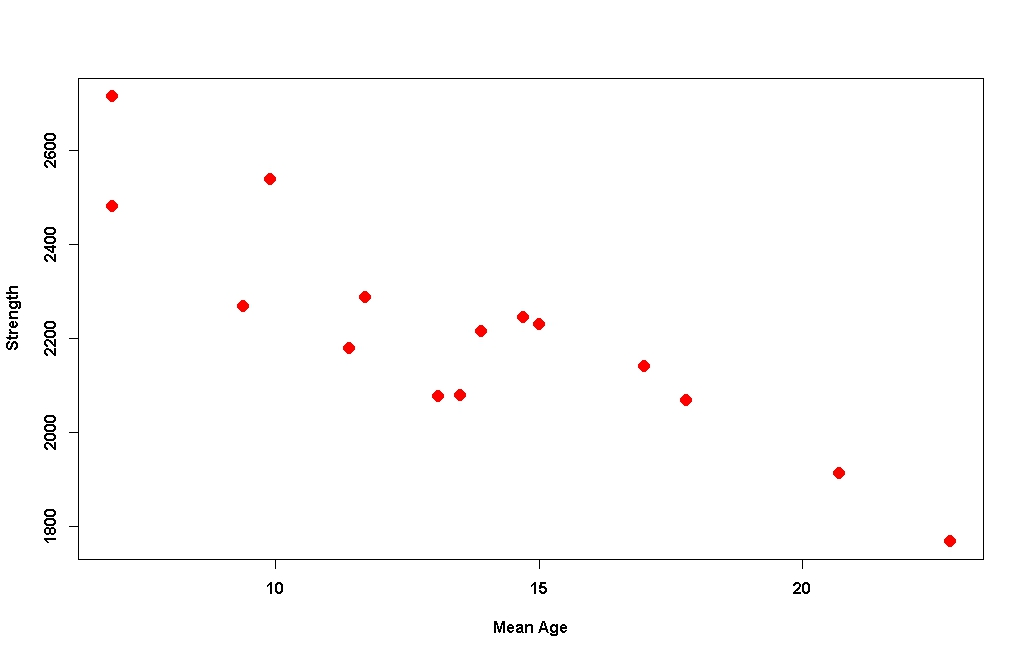
\includegraphics[scale=0.3]{12Aplot1}\\
%\end{figure}
%

%----------------------------------------------------%

\subsection{Example 1 (c)}
\begin{itemize}
	\item What sort of relationship is indicated by this scatterplot?
	\item Strong or Weak?  - Quite Strong
	\item Positive or Negative?  - Negative
	\item Linear or Non-Linear - Seems to be linear
\end{itemize}

%----------------------------------------------------%

\subsection{Example 1 (d)}
Suppose we are given the following summations
\begin{itemize}
	\item $\sum X = 213.4$
	\item $\sum X^2 =3277.82$
	\item $\sum Y = 34122$
	\item $\sum Y^2 = 78547854$
	\item $\sum XY = 472203.9$
\end{itemize}
Compute the mean values of $X$ and $Y$.

\[ \bar{x} = \frac{\sum x}{n} = \frac{213.4}{15} = 14.226 \]

Similarly $\bar{y} =  2274.8$


%----------------------------------------------------%

\subsection{Example 1 (e)}
Compute the \textbf{Sum of Squares Identities} ($S_{XX}$ , $S_{YY}$ and $S_{XY}$).\\

\bigskip
From Formula Sheet (Back of Exam Paper)
\begin{eqnarray*}
	S_{XY} &=&
	\sum x_iy_i - \frac{\sum x_i\sum y_i}{n} = \left[472203.9 - \frac{213.4 \times 34122}{15} \right]=  -13238.42\\
	S_{XX} &=&
	\sum x_i^2 - \frac{(\sum x_i)^2}{n} = \left[3277.82 - \frac{213.4^2}{15}\right] =  241.8493\\
	S_{YY} &=&
	\sum y_i^2 - \frac{(\sum y_i)^2}{n} = \left[78547854 - \frac{34122^2}{15}\right] = 927128.4\\
\end{eqnarray*}



%----------------------------------------------------%

\subsection{Example 1 (f)}
Compute the \textbf{Correlation Coefficient} $r_{XY}$

\[r_{XY} =  \frac{S_{XY}}{\sqrt{S_{XX} \times S_{YY}}} \]

\[r_{XY} =  \frac{-13238.42}{\sqrt{241.8493 \times 927128.4}} \]
Remark : $\sqrt{XY} = \sqrt{X} \times \sqrt{Y}$.
\[r_{XY} =  \frac{-13238.42}{\sqrt{241.8493} \times \sqrt{927128.4}} \]
\[r_{XY} =  \frac{-13238.42}{15.55 \times 962.87} = \frac{-13238.42}{14972.63} = -0.8841 \]

This value is consistent with our interpretation of the scatterplot: Strong Negative Linear Relationship.

%----------------------------------------------------%


\subsection{Example 1 (g)}
Calculate the least squares regression line.\\
\bigskip
The least squares regression line comprises two important estimates:
\begin{itemize}
	\item  The slope estimate $b_1$
	\item  The intercept estimate $b_0$.
\end{itemize}
The least squares regression line has the following form:

\[ \hat{y}  = b_0 + b_1x \]

$\hat{y}$ is the \textbf{predicted} value for variables Y, when given a particular value $x$ for the predictor variable X.

%----------------------------------------------------%



\subsection{Example 1 (h)}

\begin{itemize}
	\item  The slope estimate $b_1$
	
	\begin{eqnarray*}
		b_1 = \frac{S_{XY}}{S_{XX}} = \frac{-13238.42}{241.8493} = -54.738
	\end{eqnarray*}
	
	\item  The intercept estimate $b_0$.
	\begin{eqnarray*}
		b_0 = \bar{y} -b_1\bar{x} = 2274.8 - (-54.738 \times 14.226) = 3053.503
	\end{eqnarray*}
\end{itemize}

\[ \hat{y}  = 3053.503 -54.738 x \]


%----------------------------------------------------%

\subsection{Example 1 (i)}
Interpret the values of the slope and the intercept.
\begin{itemize}
	\item  The slope estimate $b_1$ :  For each additional year in age, the shear strength of the bond decreases by approximately 54 units.
	\item The Intercept estimate $b_0$ : When the age of the propellant is 0 (i.e. brand new) the strength of the bond is expected to be 3053 units.
\end{itemize}
\bigskip
What is the estimate of the mean shear strength of the bond if the mean age of the propellants is 17 weeks?

\[ \hat{y}_{(x=17)}  = 3053.503 -54.738 \times 17 = 2122.96 \]

That looks plausible, from looking back at the scatter-plot.


%----------------------------------------------------%

\subsection{Example 1 (j)}

% image
% 12plot1
%\begin{figure}
%% Requires \usepackage{graphicx}
%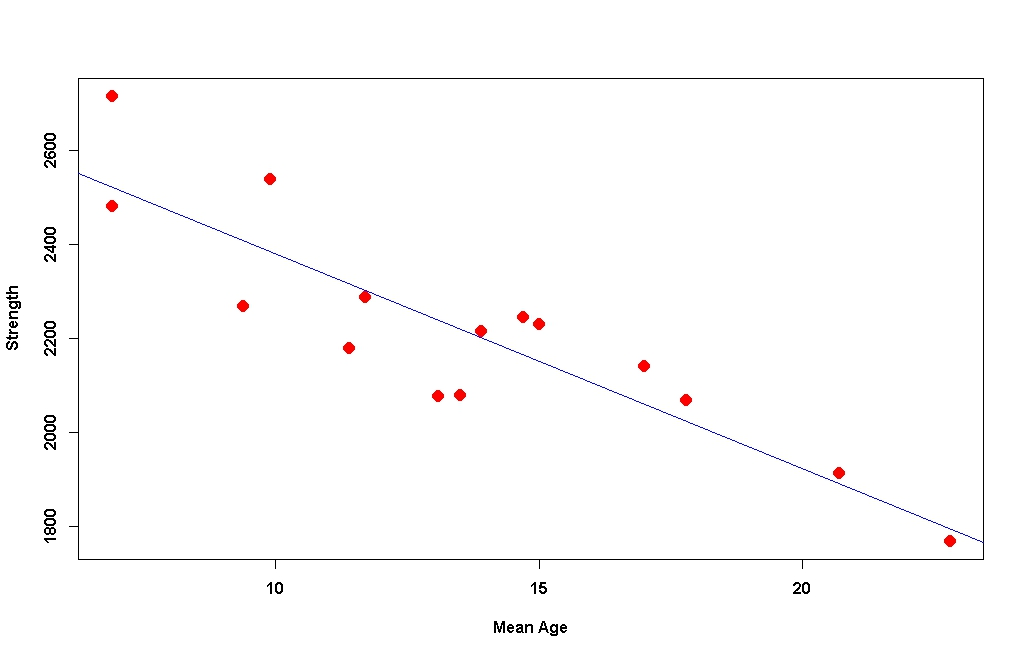
\includegraphics[scale=0.3]{12Aplot2}\\
%\end{figure}
%

%----------------------------------------------------%

\subsection{Example 2 (a)}
(Spring 2010 Q5)\newline
A wood scientist wishes to determine if there is a relationship between the number of knots in a piece of wood and its tensile strength. A random selection of 8 timber beams were analysed and the results are given in the table (next slide).

%----------------------------------------------------%

\subsection{Example 2 (b)}
\begin{center}
	\begin{tabular}{|c|c|c|}
		\hline
		% after \\: \hline or \cline{col1-col2} \cline{col3-col4} ...
		Observation &Number of knots (x) &Tensile Strength \\
		&&N.MS (y)\\ \hline
		A &5&5\\
		B &8&2.9\\
		C &4&4.9\\
		D &9&2.8\\
		E &3&6.1\\
		F &6&4.1\\
		G &4&4.8\\
		H &7&3.2\\
		\hline
	\end{tabular}
\end{center}


%----------------------------------------------------%

\subsection{Example 2 (c)}
Computing summations: recommended approach is construction of a table.\\
\begin{center}
	\begin{tabular}{|c|c|c|c|c|c|}
		\hline
		Obs&$X$&$Y$&$X^2$&$Y^2$&$XY$\\
		A &5&5&&&25      \\
		B &8&2.9&&&23.2\\
		C &4&4.9&&&19.6\\
		D &9&2.8&&&25.2\\
		E &3&6.1&&&18.3\\
		F &6&4.1&&&24.6\\
		G &4&4.8&&&19.2\\
		H &7&3.2&&&22.4\\
		(sum)&46&33.8&&&177.5\\
		
		\hline
	\end{tabular}
\end{center}


%----------------------------------------------------%

\subsection{Example 2 (d)}

Summations from previous slide.
\begin{itemize}
	\item $\sum X = 46$
	\item $\sum X^2 =296$
	\item $\sum Y = 33.8$
	\item $\sum Y^2 = 152.56$
	\item $\sum XY = 117.5$
\end{itemize}
Compute the mean values of $X$ and $Y$.

\[ \bar{x} = \frac{\sum x}{n} = \frac{46}{8} = 5.75 \]

Similarly $\bar{y} =   4.225$




\subsection{Example 2 (g)}
Compute the \textbf{Sum of Squares Identities} ($S_{XX}$ , $S_{YY}$ and $S_{XY}$).\\
\bigskip
From Formula Sheet (Back of Exam Paper)
\begin{eqnarray*}
	S_{XY} &=&
	\sum x_iy_i - \frac{\sum x_i\sum y_i}{n} = -16.85\\
	S_{XX} &=&
	\sum x_i^2 - \frac{(\sum x_i)^2}{n} = 31.5\\
	S_{YY} &=&
	\sum y_i^2 - \frac{(\sum y_i)^2}{n} = 9.755\\
\end{eqnarray*}



\subsection{Example 2 (h)}
Compute the regression estimates:
\begin{itemize}
	\item  The slope estimate $b_1$
	
	\begin{eqnarray*}
		b_1 = \frac{S_{XY}}{S_{XX}} = \frac{-16.85}{31.5} = -0.5349
	\end{eqnarray*}
	
	\item  The intercept estimate $b_0$.
	\begin{eqnarray*}
		b_0 = \bar{y} -b_1\bar{x} = 4.225 - (-0.5349 \times 5.75) = 7.300
	\end{eqnarray*}
\end{itemize}

\[ \hat{y}  = 7.300 -0.5349 x \]



%----------------------------------------------------%

\subsection{Example 2 (i)}

% image
% 12plot1
%\begin{figure}
%% Requires \usepackage{graphicx}
%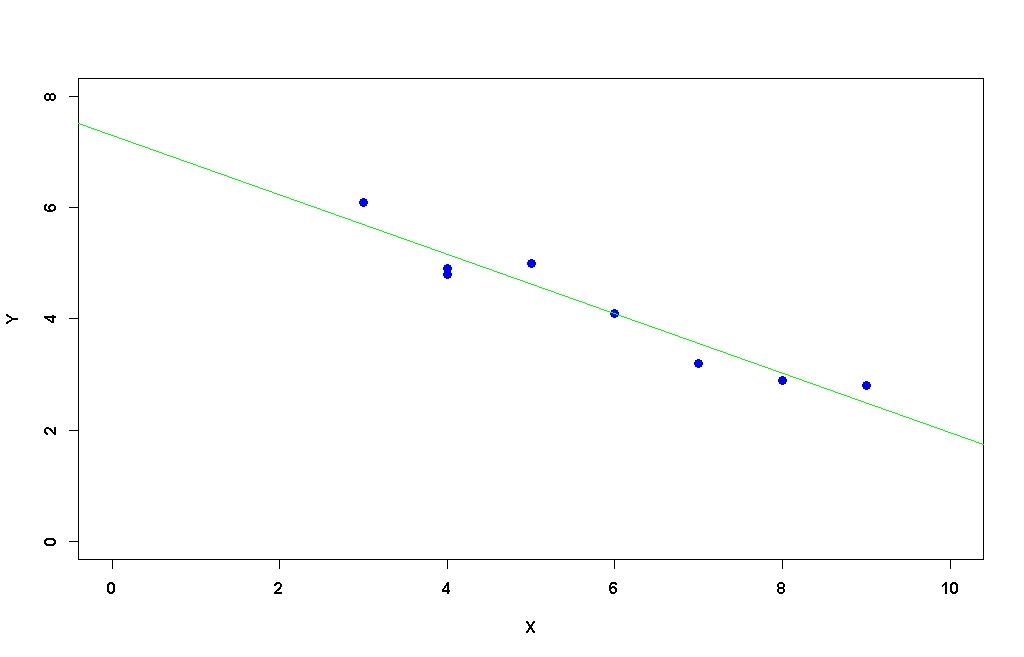
\includegraphics[scale=0.3]{12Aplot3}\\
%\end{figure}
%
%

%-----------------------------------------------------------------%

\begin{verbatim}
X=rnorm(15,12.08,sd=4)

Y=rnorm(15,2200,sd=200)

while(cor(X,Y)>(-0.875))
{
Y=rnorm(15,2200,sd=200)
}

X=round(X,1)
Y=floor(Y)


plot(X,Y,pch=17,col="blue",font.lab=2,font.axis=2,cex=1.6)
#
cor(X,Y)
sum(X)
sum(X^2)
sum(Y)
sum(Y^2)
sum(X*Y)


var(X)*(length(X)-1)
var(Y)*(length(Y)-1)
cov(X,Y)*(length(X)-1)
cor(X,Y)
coef(Y~X)
%-----------------------------------------------------------------% 

\end{verbatim}




	\section*{Linear Regression}
	\begin{itemize}
		\item Linear regression is the most widely used of all statistical techniques: it is the study of linear (i.e., straight-line) relationships between variables, usually under an assumption of normally distributed errors.
	\end{itemize}


\section{Simple Linear Regression}
\begin{itemize}
\item	We have to find the line of best fit. Before we can do this, we must assume that one
		variable is dependent on the other. 
		
	\item The theory we learn here assumes we are going to use a straight line, and not a curve of any kind, though in some disciplines (physics or finance, for example) a curve would be more appropriate.
	
	\item We have to find the line of best fit. Before we can do this, we must assume that one
	variable is dependent on the other. By convention we call the dependent variable y
	and the independent variable x. We have to work out the slope of the line, and the
	point at which it cuts the y axis.
	
	\item Again, by convention, we call these values and respectively for the population.
	
	\item The basic model is therefore given as follows.
	
	\item The model of a random variable Y, the dependent variable, which is related to random
	variable X, the independent (or predictor or explanatory) variable by the equation:
	\begin{equation}
	Y = \alpha + \beta X + \epsilon
	\end{equation}
	
	where $\alpha$ and $\beta$ are constants and $\epsilon ~ N ( 0,\sigma^2)$ , a random error term. The
	coefficients $\alpha$ and $\beta$  are theoretical values and can only be estimated from sample data.
\end{itemize}

\begin{itemize}

	\item By convention we call the dependent variable y
	and the independent variable x. We have to work out the slope of the line, and the
	point at which it cuts the y axis.
	
	\item	Again, by convention, we call these values and respectively for the population.
\end{itemize}

The estimates are generally written as $a$ and $b$.

Given a sample of bivariate data, $(x_1,y_1),(x_2,y_2) ,.........., (x_n,y_n)$, $a$ and $b$ can be
estimated. To fit a line to some data as in this case, an objective must be chosen to
define which straight line best describes the data. The most common objective is to
minimise the sum of the squared distance between the observed value of $y_i$
and the corresponding predicted value $\hat{y}_i$.

The estimated least squares regression line is written as:
$y = a + b\times x$
We can derive the formulae for $b$ and $a$.



The line is called the sample regression line of y on x.

The following example demonstrates the calculation of a and b and the use of the resultant
equation to estimate y for a given x.

\newpage


	
\begin{itemize}
\item 	The estimates are generally written as $a$ and $b$.
\item 	Given a sample of bivariate data, $(x_1,y_1),(x_2,y_2) ,.........., (x_n,y_n)$, $a$ and $b$ can be
	estimated. 
\item  To fit a line to some data as in this case, an objective must be chosen to
	define which straight line best describes the data. 
\item  The most common objective is to
	minimise the sum of the squared distance between the observed value of $y_i$
	and the corresponding predicted value $\hat{y}_i$.
\item 	The estimated least squares regression line is written as:
	$y = a + b\times x$
	We can derive the formulae for $b$ and $a$.
\item 	The line is called the sample regression line of y on x.
\item 	The following example demonstrates the calculation of a and b and the use of the resultant
	equation to estimate y for a given x.
\end{itemize}

	
%---------------------------------------------------------------------%


\section{Regression}
We consider the simplest type of regression line where there are only two
variables
\begin{itemize}
	\item  one response variable (Y)
	\item one predictor variable (X)
\end{itemize}
This is called Simple Linear Regression and the mathematical model is:
\[ Y = \beta_0 + \beta_1X + \epsilon \]

The true values of $\beta_0$ and  $\beta_1$ are almost always unknown, but are instead estimated from sample data.

%---------------------------------------------------------------------%


	\section{Ordinary least squares}
	Ordinary least squares (OLS) is a technique for estimating the unknown parameters in a linear regression model. This method minimizes the sum of squared distances between the observed responses in a set of data, and the fitted responses from the regression model.
	


		

	\section{Regression: Computing the Estimates}

	
	We are asked to calculate the following
	\begin{itemize} 
		\item an estimate for the intercept value
		\item an estimate for the slope value
	\end{itemize}
	(The chevron sign denotes that the value in question is an estimate.)
	
	
	\begin{itemize}
		\item 	We calculate the estimate for slope first.
		
		\item To calculate the estimate for the intercept, we first must determine the values for the means of X and Y (i.e  and ). We are given the values of the summations of X and Y (i.e. and ), which we divide by the number of XY pairs (‘n’). 
		
		\item 	We then construct the regression model equation , which estimate a value for Y for a  given X value. It takes the form:	
		
		\item The second part of the question will give us a particular X value and ask us to calculate a corresponding estimate for Y.
		
	\end{itemize}
	
	%-------------------------------------------------%
	\noindent \textbf{Regression Estimate}

	\begin{itemize}
		\item Slope Estimate
		\[b_1 = \frac{S_{XY}}{S_{XX}} \]
		\item Intercept Estimate
		\[b_0 = \bar{Y} - b_1\bar{X} \]
	\end{itemize}
	

	
	%-------------------------------------------------%
	\begin{framed}
		\noindent \textbf{Summation Calculations}
		\begin{multicols}{2}
			\begin{itemize}
				\item $\sum X$ - sum of the $X$ data set.
				\item $\sum Y$ - sum of the $Y$ data set.
				\item $\sum X^2$ - sum of the $X$ data set.
				\item $\sum Y^2$ - sum of the $Y$ data set.
				\item $\sum XY$ - sum of the case-wise products  of $X$ and $Y$ values.
			\end{itemize}
		\end{multicols}
	\end{framed}
	%-------------------------------------------------%

	
	%-------------------------------------------------%
	\noindent \textbf{Identities}
	\begin{multicols}{2}
	\begin{itemize}
		\item $S_{XY} = -283.8$
		\item $S_{XX} = 613.6$
		\item $S_{YY} = 148.9$
		\item $\sum(X_i)  = 318 $
		\item $\sum(Y_i)  = 61$
	\end{itemize}
	\end{multicols}

	
	
	%-------------------------------------------------%
	\noindent \textbf{Example 2 Part 1}
	
	\begin{itemize}
		\item Calculate the slope estimate for the regression equation.
		\item The slope estimate is computed using the following formula:
		\[ b_1 = \frac{\S_{XY}}{S_{XX}} \]
		\item From the values given
		\[ b_1 = \frac{-283.8}{613.6} =-0.4625 \]
		\item 
	\end{itemize}
	
	
	

	

	





\section{Regression Coefficients} Meaning of the Regression Coefficients:
\begin{itemize} \item $\beta_1$ is the slope of the regression line.
	\item It gives the average change in the response variable Y for each unit
	change in X.
	\item The slope can either be negative or positive.
	\item A positive slope of 5, for example, means that for every 1 unit increase
	in X we can expect an average 5 units increase in Y.
	\item $\beta_0$ indicates the value of Y when X is zero (only holds if the population could
	have X values of 0 - otherwise $\beta_0$ does not have a meaningful interpretation
	in the regression model).
\end{itemize}

%------------------------------------------------------- %

\textbf{Regression Least Square Estimation}
\begin{itemize}
	\item There are many straight lines that could be drawn to represent the
	relationship between X and Y.
	\item The \textbf{least squares} method is one of the methods that can be used to find
	the straight line that provides the best approximation for the relationship
	between the independent and dependent variables.
	\item This method consists of choosing estimate values of $b_0$ and $b_1$ which minimize the sum
	of the squared vertical distances measured from the data to the line.
\end{itemize}

\subsection{Regression Least Square Estimation}
The
equation of the line obtained using the least squares method is of the form:
\[ \hat{y} = b_0 + b_1x \]
where
\begin{itemize}
	\item $b_0$ = estimated intercept of the line
	\item $b_1$ = estimated slope of the line
	\item $\hat{y}$ = estimated value of the response variable
\end{itemize}

%--------------------------------------------------------------------- %

\newpage

\section{Question 5b : Simple Linear Regression}

% part i
Use the above table, give the equation of the regression line expressing pressure as a function of volume

\begin{itemize}
	\item  Intercept estimate :	 70.048
	\item Slope estimate :         -7.402
\end{itemize}

\[
Regression line  : Pres.= 70.048 - 7.402Vol. 
\]
Pres.  is the pressure estimated from the model for a certain volume. 




part ii

According to the model, what is the average effect on pressure resulting from an increase in volume of one cubic metre.


For every increase of one cubic metre in volume, the pressure is estimate to decrease by -7.402  bars.


Part iii

Using this model, estimate the air pressure when the slope is 5 metres cubed.

33.038 bars.

Part iv

The observation if the air pressure at a volume of 5 cubic metres was 19.87 bars.

Calculate the residual from the regression model corresponding to this observation

\[Residual = Estimate - Observered value = 30.038 - 19.87\]

Residual = 13.168 

Part v: Hypothesis test on the slope.


If the true value of the slope is zero, then there is no relationship between volume and pressure.

(i.e. Null hypothesis means that Pressure doesnt depend on volume).


The null and alternative hypotheses are as follows

Ho:1= 0  	 The true value of the slope is zero


The true value of the slope is not zero






Part vi
\begin{itemize}
	\item Briefly explain why the  use of linear regression to describe pressure as a funciton of voumen is inappropriate.
	
	\item Looking at the scatterplot, we can clearly see that the relationship between pressure and volume is curved (i.e. not linear). 
	
	\item Therefore linear regression is not an appropriate analysis for this data.
\end{itemize}


	
	
	

	
	\section{Regression example}
	
	In a medical experiment concerning 12 patients with a certain type of ear condition,
	the following measurements were made for blood flow (y) and auricular pressure (x):
	
%%	\begin{verbatim}
%%	x<-c(8.5, 9.8, 10.8, 11.5, 11.2, 9.6, 10.1, 13.5, 14.2, 11.8, 8.7, 6.8)
%%	y<-c(3 ,12, 10, 14, 8 ,7 ,9 ,13, 17, 10, 5 ,5)
%%	\end{verbatim}
%%	
	
	($S_x =126.5 S_{xx} =1,381.85 S_y =113 S_{yy} =1251, S_{xy} =1272.2$)
	
	
	\begin{itemize}
		\item Calculate the equation of the least-squares fitted regression line of blood flow
		on auricular pressure.
		\item Confirm the following values: Sx =126.5, Sxx =1381.85, Sy =113, Syy =1251, Sxy =1272.2.
		\item Calculate the correlation coefficient.
		
%%		\begin{verbatim}
%%		> cor(x,y)
%%		[1] 0.8521414
%%		\end{verbatim}
	\end{itemize}
	
	



\section{Retailer - Regression Example}
\begin{itemize}
	\item A study was made by a retailer to determine the relation between weekly advertising
	expenditure and sales (in thousands of pounds).
	\item Find the equation of a regression line
	to predict weekly sales from advertising.
	\item Estimate weekly sales when advertising
	costs are 35,000.
\end{itemize}


Units denominated in thousands \\(i.e. X = 40 means advertising cost of 40,000)
\begin{center}
	\begin{tabular}{|c|c|c|c|c|c|c|}
		\hline
		% after \\: \hline or \cline{col1-col2} \cline{col3-col4} ...
		Adv. Costs & 40 & 20 & 25 & 20 & 30 & 50\\
		Sales & 385& 400& 395& 365& 475& 440\\ \hline \hline
		Adv. Costs & 40 & 20 & 50 & 40 & 25 & 50\\
		Sales & 490& 420& 560& 525& 480& 510\\
		\hline
	\end{tabular}
\end{center}


%%%%%%%%%%%%%%%%%%%%%%%%%%%%%%%%%%%%%%%%%%%%%%%%%%%%%%%%%%%%%%%%%%%%%%%%%

\textbf{Regression Example}
Scatterplot: Indicates a weak positive linear relationship.
\begin{center}
	\begin{figure}
		% Requires \usepackage{graphicx}
		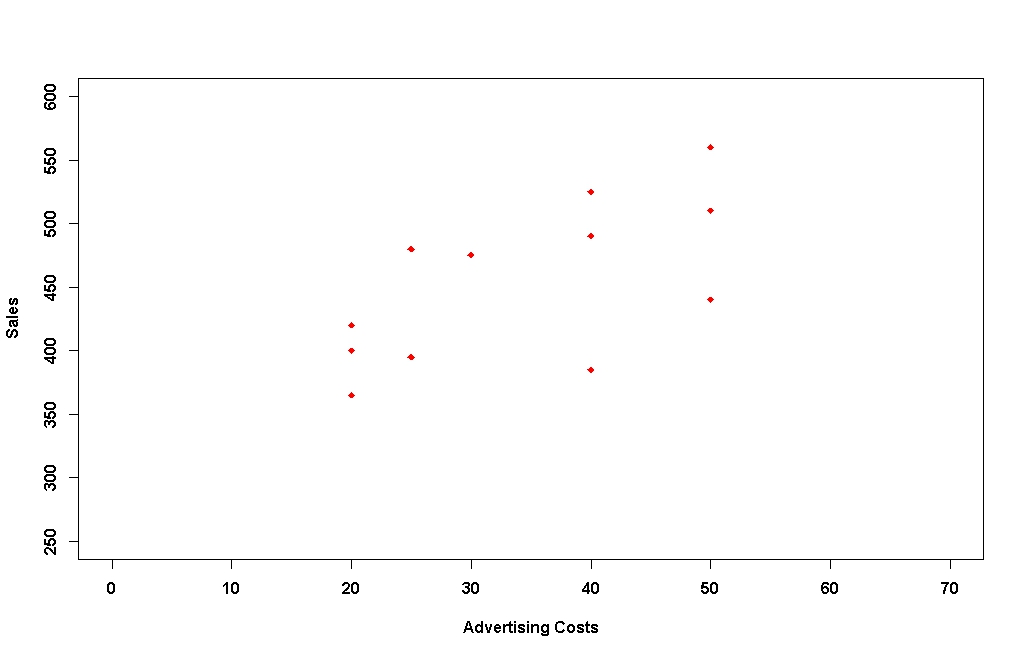
\includegraphics[scale=0.3]{images/12Bplot1.jpeg}\\
	\end{figure}
\end{center}


Summations
\begin{multicols}{2}
	\begin{itemize}
		\item $\sum X$ = 410
		\item $\sum Y$ = 5445
		\item $\sum X^2$ = 15650
		\item $\sum Y^2$ = 2512925
		\item $\sum XY$ = 191325
	\end{itemize}
\end{multicols}
Mean Values
\begin{itemize}
	\item $\bar{x}$ = 34.16
	\item $\bar{y}$ = 453.75
\end{itemize}


%%%%%%%%%%%%%%%%%%%%%%%%%%%%%%%%%%%%%%%%%%%%%%%%%%%%%%%%%%%%%%%%%%%%%%%%%

\textbf{Regression Example}
Sums of Squares Identities
\begin{itemize}
	\item $S_{XX}$ = 1641.67
	\item $S_{YY}$ = 42256.25
	\item $S_{XY}$ = 5287.5
\end{itemize}
Pearson's Correlation Estimate
\[ r_{XY} = \frac{S_{XY}}{\sqrt{S_{XX} \times S_{YY}}} = \frac{5287.5}{\sqrt{1641.67 \times 42256.25}} = 0.6348 \]

Weak to strong positive linear relationship.

%%%%%%%%%%%%%%%%%%%%%%%%%%%%%%%%%%%%%%%%%%%%%%%%%%%%%%%%%%%%%%%%%%%%%%%%%

\textbf{Regression Example}
Regression Coefficients
\begin{itemize}
	\item Slope Estimate $b_1$
	\[b_1 = \frac{S_{XY}}{S_{XX}} = {5287.5 \over 1641.67} = 3.221\]
	\item Intercept Estimate $b_0$ = $\bar{y} - b_1 \times \bar{x}$ = $453.75-(3.221\times 34.16)$ = 343.70
\end{itemize}
Regression Equation
\[ \hat{y} = 343.70 + 3.221x \]


%%%%%%%%%%%%%%%%%%%%%%%%%%%%%%%%%%%%%%%%%%%%%%%%%%%%%%%%%%%%%%%%%%%%%%%%%

\textbf{Regression Example}
\begin{center}
	\begin{figure}
		% Requires \usepackage{graphicx}
		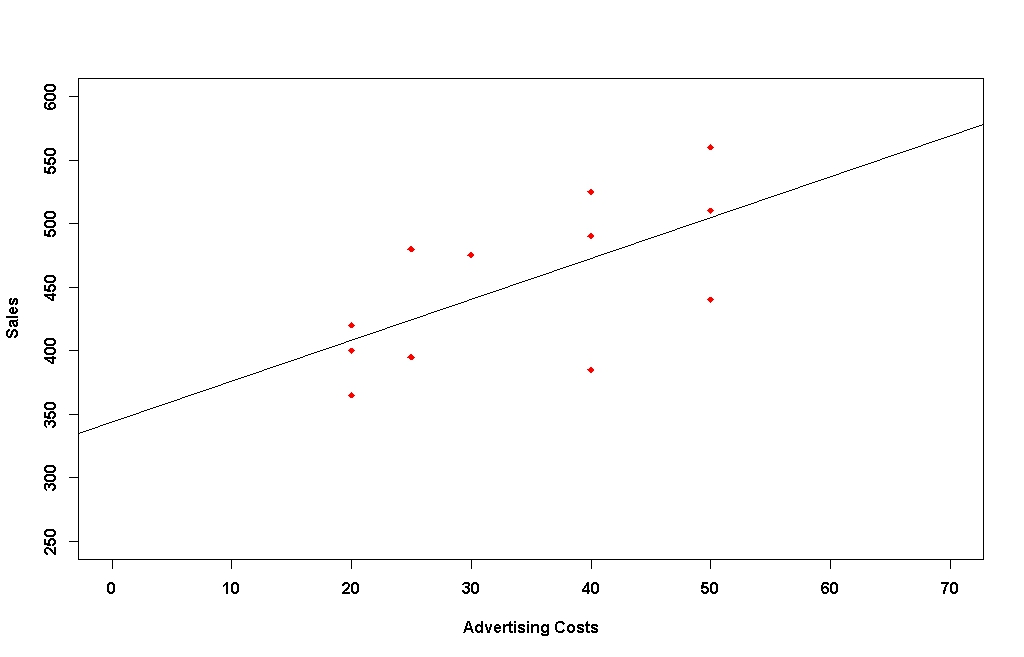
\includegraphics[scale=0.3]{images/12Bplot2.jpeg}\\
	\end{figure}
\end{center}





%-------------------------------------------------%
\noindent \textbf{Regression Estimate}
\begin{itemize}
	\item Intercept Estimate
	\item Slope Estimate
\end{itemize}

%-------------------------------------------------%
\noindent \textbf{Summation Calculations}
\begin{itemize}
	\item $\sum X$ - sum of the $X$ data set.
	\item $\sum Y$ - sum of the $Y$ data set.
	\item $\sum X^2$ - sum of the $X$ data set.
	\item $\sum Y^2$ - sum of the $Y$ data set.
	\item $\sum XY$ - sum of the case-wise products  of $X$ and $Y$ values.
\end{itemize}

\subsubsection{Regression Example}
Scatterplot: Indicates a weak positive linear relationship.
\begin{center}
	\begin{figure}
		% Requires \usepackage{graphicx}
		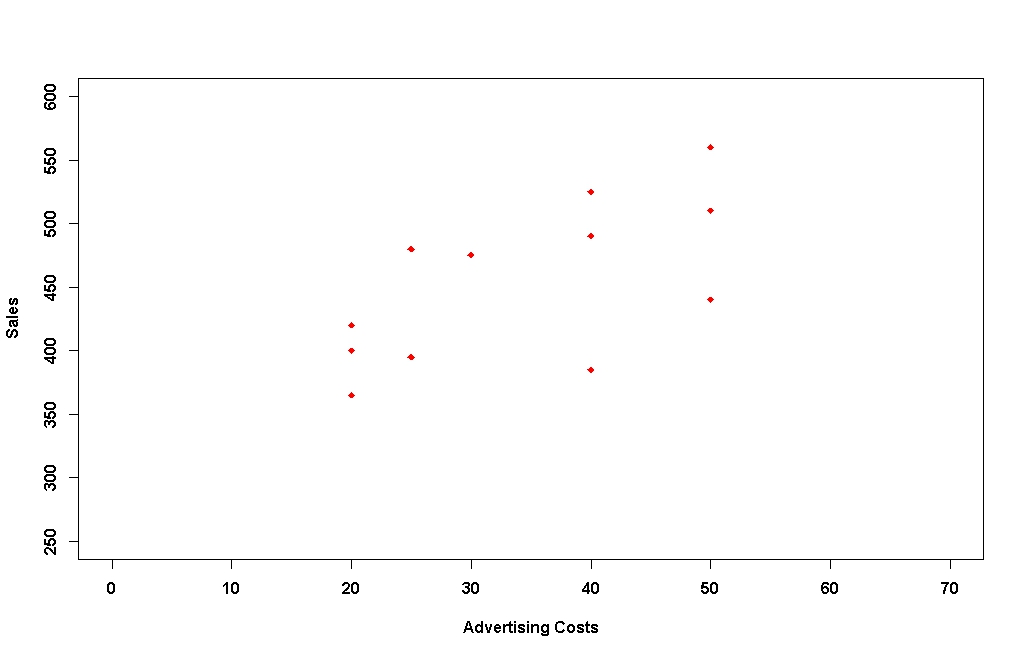
\includegraphics[scale=0.3]{images/12Bplot1.jpeg}\\
	\end{figure}
\end{center}

%%%%%%%%%%%%%%%%%%%%%%%%%%%%%%%%%%%%%%%%%%%%%%%%%%%%%%%%%%%%%%%%%%%%%%%%%


Summations
\begin{itemize}
	\item $\sum X$ = 410
	\item $\sum Y$ = 5445
	\item $\sum X^2$ = 15650
	\item $\sum Y^2$ = 2512925
	\item $\sum XY$ = 191325
\end{itemize}
Mean Values
\begin{itemize}
	\item $\bar{x}$ = 34.16
	\item $\bar{y}$ = 453.75
\end{itemize}


%%%%%%%%%%%%%%%%%%%%%%%%%%%%%%%%%%%%%%%%%%%%%%%%%%%%%%%%%%%%%%%%%%%%%%%%%

Sums of Squares Identities
\begin{itemize}
	\item $S_{XX}$ = 1641.67
	\item $S_{YY}$ = 42256.25
	\item $S_{XY}$ = 5287.5
\end{itemize}
Pearson's Correlation Estimate
\[ r_{XY} = \frac{S_{XY}}{\sqrt{S_{XX} \times S_{YY}}} = \frac{5287.5}{\sqrt{1641.67 \times 42256.25}} = 0.6348 \]

Weak to strong positive linear relationship.

%%%%%%%%%%%%%%%%%%%%%%%%%%%%%%%%%%%%%%%%%%%%%%%%%%%%%%%%%%%%%%%%%%%%%%%%%

Regression Coefficients
\begin{itemize}
	\item Slope Estimate $b_1$ = $S_{XY}$/$S_{XX}$ = 5287.5 / 1641.67 = 3.221
	\item Intercept Estimate $b_0$ = $\bar{y} - b_1 \times \bar{x}$ = $453.75-(3.221\times 34.16)$ = 343.70
\end{itemize}
Regression Equation
\[ \hat{y} = 343.70 + 3.221x \]


%%%%%%%%%%%%%%%%%%%%%%%%%%%%%%%%%%%%%%%%%%%%%%%%%%%%%%%%%%%%%%%%%%%%%%%%%

\begin{center}
	\begin{figure}
		% Requires \usepackage{graphicx}
		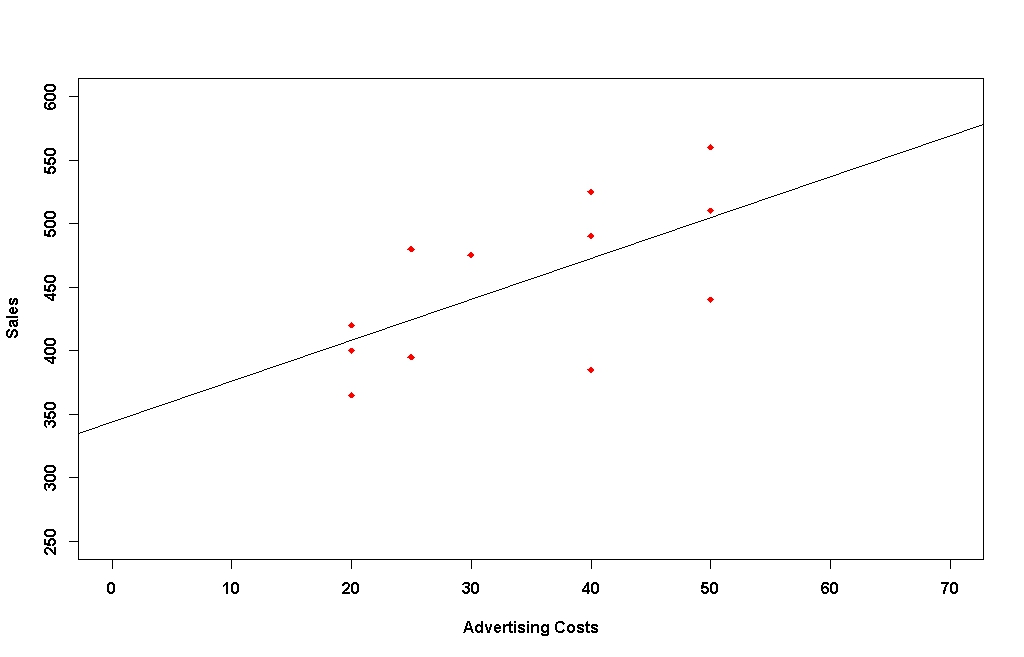
\includegraphics[scale=0.3]{images/12Bplot2.jpeg}\\
	\end{figure}
\end{center}

%%%%%%%%%%%%%%%%%%%%%%%%%%%%%%%%%%%%%%%%%%%%%%%%%%%%%%%%%%%%%%%%%%%%%%%%%


Estimate weekly sales when advertising costs are 35,000 (i.e X=35).
\[ \hat{y} = 343.70 + 3.221x \]

\[ \hat{y}_{X=35} = 343.70 + 3.221(35)  = 456.4 \]

When the advertising costs are 35,000, the expected sales are predicted to be 456,400.

Estimate weekly sales when advertising costs are 40,000 (ie. X=40).


\[ \hat{y}_{X=35} = 343.70 + 3.221(40)  = 472.54 \]

When the advertising costs are 40,000, the expected sales are predicted to be 472,540.


\subsubsection{Regression Example}

Predicted and Observed values
\begin{itemize}
	\item In simple linear regression, we predict scores on one variable from the scores on a second variable.
	\item In the last example, we predicted the value of sales to be 472.54 the costs were X=40.
	\item In fitting the model, we used three observations when the value of X was 40 (i.e. Y = 385,490,525)
	\item These are observed values, used to compute the model, and are distinct from predicted values $\hat{y}$.
	\item The predicted values are estimates for future observations
	\item The difference between an observed value and it's corresponding predicted value is known as a \textbf{\textit{residual}}.
	\[e_i = y_i-\hat{y}_i \]
	\item As there are three observations at X=40, there are three residuals.
\end{itemize}



		\section{Divorce Rate - Regression example}
	
	A survey was conducted in 9 areas of the USA to investigate the relationship between
	\textbf{\textit{divorce rate (y)}} and \textbf{\textit{residential mobility (x)}}. Divorce rates in the annual number per 1000 in the population
	and the residential mobility is measured by the percentage of the population that moved house in the last
	five years.
	
	\begin{center}
		\begin{tabular}{|c|c|c|c|c|c|c|c|c|c|}
			\hline
			Area & 1 & 2 & 3 & 4 & 5 & 6 & 7 & 8 & 9  \\ \hline 
			x & 40 & 38 & 46 & 49 & 47 & 43 & 51 & 57 & 55\\ \hline
			y & 3.9 & 3.4 & 5.2 & 4.8 & 5.6 & 5.8 & 6.6 & 7.6 & 5.8\\
			\hline
		\end{tabular}
	\end{center}
	
	
	
	\begin{itemize}
		\item Check that the following statements are correct.
		
		\begin{itemize}
			\item[$\bullet$] sum of x data = 426
			\item[$\bullet$] sum of squares of x data = 20494
			\item[$\bullet$]sum of y data = 48.7
			\item[$\bullet$] sum of squares of y data = 276.81
			\item[$\bullet$] sum of products of x and y data = 2361
		\end{itemize}
		
		\item Derive the estimates for the slope and intercept of the regression line.
		\item Estimate the divorce rate for areas that has a residential mobility of 39 and 60 respectively.
		\item Which of these estimates is likely to be more accurate? Why?
		
	\end{itemize}
	
	
	
\newpage	


\section*{Ansombe's Quartet}
\begin{tabular}{||c|c||c|c||c|c||c|c||}
	\hline
	Set 1 	&		&	Set 2	&		&	Set 3	&		&	Set 4	&		\\
	x	&	y	&	x	&	y	&	x	&	y	&	x	&	y	\\
	10	&	8.04	&	10	&	9.14	&	10	&	7.46	&	8	&	6.58	\\
	8	&	6.95	&	8	&	8.14	&	8	&	6.77	&	8	&	5.76	\\
	13	&	7.58	&	13	&	8.74	&	13	&	12.74	&	8	&	7.71	\\
	9	&	8.81	&	9	&	8.77	&	9	&	7.11	&	8	&	8.84	\\
	11	&	8.33	&	11	&	9.26	&	11	&	7.81	&	8	&	8.47	\\
	14	&	9.96	&	14	&	8.1	&	14	&	8.84	&	8	&	7.04	\\
	6	&	7.24	&	6	&	6.13	&	6	&	6.08	&	8	&	5.25	\\
	4	&	4.26	&	4	&	3.1	&	4	&	5.39	&	19	&	12.5	\\
	12	&	10.84	&	12	&	9.13	&	12	&	8.15	&	8	&	5.56	\\
	7	&	4.82	&	7	&	7.26	&	7	&	6.42	&	8	&	7.91	\\
	5	&	5.68	&	5	&	4.74	&	5	&	5.73	&	8	&	6.89	\\
	\hline
\end{tabular}






{Regression : Least Square Estimation}
It can be shown, using differential calculus that the values of $b_0$
and $b_1$ that best estimate the true parameters $\beta_0$ and $\beta_1$ are:

\[ b_1 = \frac{S_{XY}}{S_{XX}}\]
and
\[ b_0 = \bar{y} - b_1 \bar{x} \]

$\bar{x}$ and $\bar{x}$ are the sample means of X and Y respectively.


			\section*{May 2013 Question 6b Correlation and Regression }
			Calculate the correlation coefficient and interpret the value.
			\begin{tabular}{|c|c|c|}
				\hline Residence	& X	  & Y \\ 
				\hline  &  &  \\ 
				\hline  &  &  \\ 
				\hline 
			\end{tabular} 
			
			%-------------------------------------------------%
			
			\section*{Theory Components}
			\begin{itemize}
				\item Distinguish between a bimodal distribution and a unimodal distribution
				\item Compare and contrast interval and ordinal data.
			\end{itemize}







\subsubsection{Regression Example}
Scatterplot: Indicates a weak positive linear relationship.
\begin{center}
	\begin{figure}
		% Requires \usepackage{graphicx}
		\includegraphics[scale=0.3]{images/12Bplot3.jpeg}\\
	\end{figure}
\end{center}



\subsubsection{Regression Example}

Predicted and Observed Values

\begin{center}
	\begin{tabular}{|c|c|c|c|}
		\hline
		% after \\: \hline or \cline{col1-col2} \cline{col3-col4} ...
		X & Y& $\hat{y}$ & $e_i$ \\
		40 &385 &472.54 &-87.54\\
		40 &490 &472.54 & 17.46\\
		40 &525 &472.54 & 52.46\\
		\hline
	\end{tabular}
\end{center}



\subsubsection{Important Assumptions of Least Squares Regression}
It is assumed that
\begin{itemize}
	\item The residuals are independent and normally distributed,
	\item The residuals are normally distributed with mean zero,
	\item The residuals is independent of X.
	\item The variance of residuals is consistent across the range of X (Heteroscedascity).
\end{itemize}
If these assumptions are not met, then Least Squares regression is not appropriate as a solution, and other alternatives must be used (Not Part of Course).

\subsubsection{Extrapolation}
\begin{itemize}
	\item
	Whenever a linear regression model is fit to a group of data, the range of the data should be carefully observed. \item  Attempting to use a regression equation to predict values outside of this range is often inappropriate, and may yield incredible answers. \item This practice is known as extrapolation. \item Consider, for example, a linear model which relates weight gain to age for young children. \item Applying such a model to adults, or even teenagers, would be absurd, since the relationship between age and weight gain is not consistent for all age groups.
\end{itemize}

			
			\section*{May 2012 Question 2 Correlation and Regression}
			\begin{itemize}
				\item The sample size $n$ = 10.
				\item The \textbf{\textit{independent}} variable, usually denoted $x$, is the "cause variable" or "predictor variable".
				\item The \textbf{\textit{dependent}} variable, usually denoted $y$, is the "effect variable".
				\item Here the Maths achievement test score is the independent variable and the final grade in statistics is the dependent variable.
				\item A big hint is given in the notation of the question.
			\end{itemize}
			
			% X = c(39,43,21,64,57,47,28,75,34,52)
			% Y = c(65,78,52,82,92,89,73,98,56,75)

	
	
	\textbf{Regression Example}
	Estimate weekly sales when advertising costs are 35,000 (i.e X=35).
	\[ \hat{y} = 343.70 + 3.221x \]
	
	\[ \hat{y}_{(X=35)} = 343.70 + 3.221(35)  = 456.4 \]
	
	When the advertising costs are 35,000, the expected sales are predicted to be 456,400.
	
	Estimate weekly sales when advertising costs are 40,000 (ie. X=40).
	
	
	\[ \hat{y}_{(X=40)} = 343.70 + 3.221(40)  = 472.54 \]
	
	When the advertising costs are 40,000, the expected sales are predicted to be 472,540.
	
	
	\textbf{Regression Example}
	
	Predicted and Observed values
	\begin{itemize}
		\item In simple linear regression, we predict scores on one variable from the scores on a second variable.
		\item In the last example, we predicted the value of sales to be 472.54 the costs were X=40.
		\item In fitting the model, we used three observations when the value of X was 40 (i.e. Y = 385,490 and 525)
		\item These are observed values, used to compute the model, and are distinct from predicted values $\hat{y}$.
		\item The predicted values are estimates for future observations
		\item The difference between an observed value and it's corresponding predicted value is known as a \textbf{\textit{residual}}.
		\[e_i = y_i-\hat{y}_i \]
		\item As there are three observations at X=40, there are three residuals.
	\end{itemize}
	
	
%	%%%%%%%%%%%%%%%%%%%%%%%%%%%%%%%%%%%%%%%%%%%%%%%%%%%%%%%%%%%%%%%%%%%%%%%%%
%	
%	\textbf{Regression Example}
%	Scatterplot: Indicates a weak positive linear relationship.
%	\begin{center}
%		\begin{figure}
%			% Requires \usepackage{graphicx}
%			\includegraphics[scale=0.3]{12Bplot3.jpeg}\\
%		\end{figure}
%	\end{center}
%	
	
	

	
	\begin{center}
		\begin{tabular}{|c|c|c|c|}
			\hline
			% after \\: \hline or \cline{col1-col2} \cline{col3-col4} ...
			X & Y& $\hat{y}$ & $e_i$ \\
			40 &385 &472.54 &-87.54\\
			40 &490 &472.54 & 17.46\\
			40 &525 &472.54 & 52.46\\
			\hline
		\end{tabular}
	\end{center}
	
	
	
	\textbf{Important Assumptions of Least Squares Regression}
	It is assumed that
	\begin{itemize}
		\item The residuals are independent and normally distributed,
		\item The residuals are normally distributed with mean zero,
		\item The residuals is independent of X.
		\item The variance of residuals is consistent across the range of X (Heteroscedascity).
	\end{itemize}
	If these assumptions are not met, then Least Squares regression is not appropriate as a solution, and other alternatives must be used (Not Part of Course).
	
	%%%%%%%%%%%%%%%%%%%%%%%%%%%%%%%%%%%%%%%%%%%%%%%%%%%%%%%%%%%%%%%%%%%%%%%%%
	
	\textbf{Extrapolation}
	\begin{itemize}
		\item
		Whenever a linear regression model is fit to a group of data, the range of the data should be carefully observed. \item  Attempting to use a regression equation to predict values outside of this range is often inappropriate, and may yield incredible answers. \item This practice is known as extrapolation. \item Consider, for example, a linear model which relates weight gain to age for young children. \item Applying such a model to adults, or even teenagers, would be absurd, since the relationship between age and weight gain is not consistent for all age groups.
	\end{itemize}
	
	
	






%-------------------------------------------------%
% R Code
%
% X = c(10, 15, 20, 25, 30, 35, 40)
% Y = c(11, 19, 34, 52, 58, 81, 109)
% plot(X,Y,pch=18,col="red",font.lab=2,main="Scatter Plot of X and Y")
% cor(X,Y) =0.9830478



%---------------------------------------------------------- %
\subsection*{Sums of Squares Identities}
Before we do anything, We need to compute the following sums of squares identities
\begin{itemize}
	\item $s_{xx}$
	\item $s_{yy}$
	\item $s_{xy}$
\end{itemize}
\subsection*{Calculation 1}
\[ s_{xx}  = \sum(x^2) - \frac{\sum(x)^2}{n} \]
\[ s_{xx}  = 23.634 - \frac{\sum(x)^2}{10} \]

\subsection*{Calculation 2}
\[ s_{yy}  = \sum(y^2) - \frac{\sum(y)^2}{n} \]
%\[ s_{xx}  = 23.634 - \frac{\sum(x)^2}{10} \]


\subsection*{Calculation 3}
\[ s_{xy}  = \sum(xy) - \frac{\sum(x)\times \sum{y}}{n} \]
%\[ s_{xx}  = 23.634 - \frac{\sum(x)^2}{10} \]

%------------------------------------------------------------%

\subsection*{Part iv - Prediction}
\begin{itemize}
	\item Suppose the regression equation is as follows
	\[ \hat{y} = 40.78424 + 0.76556 x \]
	\item If a student scored 5 marks on the achievement test (i.e. $x=5$), predict the students statistics grade.
	
	\[ \hat{y}_{(x=5)} = 40.78424 + (0.76556 \times 5) \]
	
	\item Solving using a calculator we get
	\[ \hat{y}_{(x=5)} = 44.61204 \]
	
	\item The score should be approximately 44.61.
\end{itemize}




%-------------------------------------------------%
%MA4104 Q4A Ana Magadalina 2010
%-------------------------------------------------%
\noindent \textbf{Example 2}



% X = c(40,28,34,27,21,38,19,45,31,35)
% Y = c(1,6,6,9,12,4,13,2,5,3)


%-------------------------------------------------%
\noindent \textbf{Identities}
\begin{itemize}
	\item $S_{XY} = -283.8$
	\item $S_{XX} = 613.6$
	\item $S_{YY} = 148.9$
	\item $\sum(X_i)  = 318 $
	\item $\sum(Y_i)  = 61$
\end{itemize}


%-------------------------------------------------%
\noindent \textbf{Example 2 Part 1}

\begin{itemize}
	\item Calculate the correlation coefficient and interpret its value.
	\item The correlation coefficient is computed using the following formula:
	\[ r_{X,Y} = \frac{\S_{XY}}{\sqrt{\S_{XX}\S_{YY}}} \]
	\item From the values given
	\[ r_{X,Y} = \frac{-283.8}{\sqrt{(613.6)(148.9)}} = -0.9389 \]
	\item Very strong negative linear relationship
	
	\item Calculate the slope estimate for the regression equation.
	\item The slope estimate is computed using the following formula:
	\[ b_1 = \frac{\S_{XY}}{S_{XX}} \]
	\item From the values given
	\[ b_1 = \frac{-283.8}{613.6} =-0.4625 \]
	\item 
\end{itemize}



%-------------------------------------------------%



\section{Regression}

The argument to lm is a model formula in which the tilde symbol
(~) should be read as ``described by”.


This was seen several times earlier, both in connection with
boxplots and stripcharts and with the t and Wilcoxon tests.



\section{Multiple Linear Regression}
The \texttt{lm()} function handles much more
complicated models than simple linear regression. There can be many other things besides a dependent and a descriptive variable in a model formula.

A multiple linear regression analysis (which we discuss in Chapter
11) of, for example, y on x1, x2, and x3 is specified as $y ~ x1 +
x2 + x3$.


This is an F test for the hypothesis that the regression coefficient is zero. This test is not really interesting in a
simple linear regression analysis since it just duplicates information already given—it becomes more interesting when there is more than one explanatory variable.







\section*{Linear Regression}
\begin{itemize}
	\item Linear regression is the most widely used of all statistical techniques: it is the study of linear (i.e., straight-line) relationships between variables, usually under an assumption of normally distributed errors.
\end{itemize}

\subsection{Regression}

\begin{verbatim}
> lm(short.velocity~blood.glucose)
\end{verbatim}





\textbf{Least Squares}
The method of least squares is a criterion for fitting a specified model to observed data.
For example, it is the most commonly used method of defining a straight line through a set of points on a scatterplot.




%---------------------------------------------------------------------%

\subsection{Types of Regression}

\begin{itemize}
	\item \textbf{Simple Linear Regression}
	Simple linear regression aims to find a linear relationship between a response variable and a possible predictor variable by the method of least squares.
	
	
	
	\item \textbf{Multiple Regression}
	Multiple linear regression aims is to find a linear relationship between a response variable and several possible predictor variables.
	
	
	
	\item \textbf{Nonlinear Regression}
	Nonlinear regression aims to describe the relationship between a response variable and one or more explanatory variables in a non-linear fashion.
\end{itemize}

%---------------------------------------------------------------------%

\textbf{Residual}
Residual (or error) represents unexplained (or residual) variation after fitting a regression model.
It is the difference (or left over) between the observed value of the variable and the value suggested by the regression model.


%---------------------------------------------------------------------%




The line is called the sample regression line of y on x.

The following example demonstrates the calculation of a and b and the use of the resultant
equation to estimate y for a given x.






%------------------------------------------------------------------------------------------------%
\subsection{R square}
The model with the highest R2 and adjusted R2  is the preferable of all candidate models
The quadratic model is the preferable model in that case.







%---------------------------------------------------------------------%

\section{Example}

The US Olympic committee are interested in determining if there is a relationship between the experience of a coach and the number of medals won in the Olympics. A random selection of 8 coaches were analyzed and the results are given in the Table below.
\begin{itemize}
	\item Predictor: Average Years Coaching Experience (x)	
	\item Response : Average Number of Medals Won (y)
\end{itemize}
\begin{center}
	
	\begin{tabular}{|c|c|c|c|c|c|c|c|c|}
		\hline
		% after \\: \hline or \cline{col1-col2} \cline{col3-col4} ...
		Coach & A & B & C & D & E & F & G & H \\
		Experience & 5 & 8 & 4 & 9 & 3 & 6 & 4 & 7\\
		Average Medals &4.0 & 6.9&3.9&7.8&2.7&6.1&4.4&6.2\\
		\hline
	\end{tabular}
\end{center}




{Example : Summations}
\begin{center}
	\begin{tabular}{|c|c|c|c|c|c|}
		\hline
		% after \\: \hline or \cline{col1-col2} \cline{col3-col4} ...
		Case &	X	&	Y	&	XY	&	$X^2$	&	$Y^2$	\\  \hline
		A	&	5	&	4	&	20	&	25	&	16	\\
		B	&	8	&	6.9	&	55.2	&	64	&	47.61	\\
		C	&	4	&	3.9	&	15.6	&	16	&	15.21	\\
		D	&	9	&	7.8	&	70.2	&	81	&	60.84	\\
		E	&	3	&	2.7	&	8.1	&	9	&	7.29	\\
		F	&	6	&	6.1	&	36.6	&	36	&	37.21	\\
		G	&	4	&	4.4	&	17.6	&	16	&	19.36	\\
		H	&	7	&	6.2	&	43.4	&	49	&	38.44	\\ \hline
		(sum)	&	46	&	42	&	266.7	&	296	&	241.96	\\ \hline
	\end{tabular}
\end{center}



{Example}
Compute the Regression Equation, given that
\begin{itemize}
	\item $\sum xy = 266.7 $
	\item $\sum x^2 = 296 $
	\item $\sum x = 46$	
	\item $\sum y =  42$	
	\item $\sum y^2 = 241.96$
\end{itemize}


{Calculations}
\begin{itemize}
	\item\item $S_{XY}$
	\[ S_{XY} = \sum xy - \frac{(\sum x)\times (\sum y)}{n} = 266.7 - \frac{46 \times 42}{8} \]
	\[ S_{XY} = 266.7-241.5  = 25.2 \]
	\item $S_{XX}$
	\[ S_{XX} = \sum x^2 - \frac{(\sum x)^2}{n} = 296 - \frac{46 ^2}{8}\]
	\[ S_{XX} = 296 - 264.5 = 31.5 \]
	
	\item $S_{YY}$
	\[ S_{YY} = \sum y^2 - \frac{(\sum y)^2}{n} = 241.96- \frac{42^2}{8} \]
	\[ S_{YY} = 241.96 - 220.5 =  21.46 \]
\end{itemize}

%------------------------------------------%


{Calculations}
\begin{itemize}
	\item The Slope Estimate is therefore
	\[ b_1 = \frac{S_{XY}}{S_XX} = \frac{25.2}{31.5} =  0.8 \]
	\item The mean values of X and Y are computed as follows
	\[ \bar{X}  = \frac{\sum x}{n} = \frac{46}{8} = 5.75 \]
	\[ \bar{Y}  = \frac{\sum y}{n} = \frac{42}{8} = 5.25 \]
	\item The Intercept Estimate 
	\[ b_0 = \bar{y} - b_1 \bar{x} = 5.25 - (0.8\times 5.75) =0.65 \] 
\end{itemize}

%------------------------------------------%


{Calculations}
\begin{itemize}
	\item $y$ is an observed value at some value of x,
	\item $\hat{y}$ is a predicted value for some value of x.
\end{itemize}

\[ \hat{y} = b_0 + b_1x \]
\[ \hat{y} = 0.65 + 0.8x \]



{Calculations}
Suppose we wish to make a prediction as to how many medals, on average, a coach with five years experience would win. 
Here let $x=5$
\[ \hat{y} = 0.65 + 0.8(5) = 4.65\]

\section{Types of Regression}

\begin{itemize}
	\item \textbf{Simple Linear Regression}
	Simple linear regression aims to find a linear relationship between a response variable and a possible predictor variable by the method of least squares.
	
	
	
	\item \textbf{Multiple Regression}
	Multiple linear regression aims is to find a linear relationship between a response variable and several possible predictor variables.
	
	
	
	\item \textbf{Nonlinear Regression}
	Nonlinear regression aims to describe the relationship between a response variable and one or more explanatory variables in a non-linear fashion.
\end{itemize}


%---------------------------------------------------------------------%


					\end{document} 